\documentclass[a4paper,twoside,zihao=-4]{ctexrep}

\usepackage[style=utils/gb7714-2015ay,backend=biber]{biblatex}
\usepackage{fancyhdr}%引入页眉页脚宏
\usepackage{array}
\usepackage{graphicx}%图像处理宏
\usepackage{geometry}%页面设置宏
\usepackage{fontspec}
\usepackage{indentfirst}%缩进宏
\usepackage[bookmarksopen=true,bookmarksnumbered=true]{hyperref}%目录跳转宏
\usepackage{xcolor}%代码高亮宏
\usepackage{listings}%代码插入宏
\usepackage[titles]{tocloft}%目录设置宏
\usepackage{booktabs}%设置表格
\usepackage{caption}%标题设置宏
\usepackage{amsmath}%数学宏包
\addbibresource{refs/thesis-ref.bib}%参考文献数据库文件

%ctex宏样式全局设置
\ctexset{
	chapter = {
		number =  \arabic{chapter},
		format = \centering \zihao{3} \heiti,
		fixbeforeskip = true,
		beforeskip = 7.2pt,
		afterskip = 7.2pt,
		pagestyle = mainbodyhd
	},
	section= {
		format += \raggedright \zihao{4},
		afterskip = 7.2pt,
	},
	subsection={
		format += \raggedright \zihao{-4} \songti \textbf,
		afterskip = 7.2pt,
	},
	subsubsection/format +=  \raggedright \zihao{-4},
	contentsname = 目 \ 录,
}

%空白页命令
\newcommand\blankpage{
	\newpage
	~\thispagestyle{empty}
	\newpage
}

%页眉页脚样式
\newcommand\hfstyle[1]{\songti \small{#1}}
%定义字体Arial
\newfontfamily{\myarial}{Arial}
%listings宏代码样式设置
\lstset{
	columns=flexible,
	numbers=none,
	basicstyle=\myarial \normalsize,
	keywordstyle=\color{blue!70}, 
	commentstyle=\color{red!50!green!50!blue!50},
	frame=shadowbox,
	rulesepcolor=\color{red!20!green!20!blue!20},
	tabsize = 2
}

%caption设置
%caption设置
\DeclareCaptionLabelFormat{figureminus}{#1\thechapter-\arabic{figure}}
\DeclareCaptionLabelFormat{tableminus}{#1\thechapter-\arabic{table}}
\DeclareCaptionFont{heiti}{\heiti}
\captionsetup[figure]{
	font = {small,heiti},
	labelsep = space,
	labelformat = figureminus,
}
\captionsetup[table]{
	font = {small,heiti},
	labelsep = space,
	labelformat = tableminus,
}

\hypersetup{hidelinks}%设置跳转链接样式
\geometry{top=3cm,bottom=2cm,left=2.5cm,right=2.5cm}%设置纸张
\setmainfont{Times New Roman}%设置默认应为字体
%设置目录样式并加上点
\renewcommand{\cftdot}{$\cdot$}
\renewcommand{\cftdotsep}{1.5}
\setlength{\cftbeforechapskip}{10pt}

\renewcommand{\cftchapleader}{\cftdotfill{\cftchapdotsep}}
\renewcommand{\cftchapdotsep}{\cftdotsep}

\makeatletter
\renewcommand{\numberline}[1]{%
	\settowidth\@tempdimb{#1\hspace{0.5em}}%
	\ifdim\@tempdima<\@tempdimb%
	\@tempdima=\@tempdimb%
	\fi%
	\hb@xt@\@tempdima{\@cftbsnum #1\@cftasnum\hfil}\@cftasnumb}
\makeatother

%设置目录页眉页脚
\fancypagestyle{cataloguehd}{
	\fancyhf{}
	\fancyfoot[C]{\small \thepage}
	\renewcommand{\headrulewidth}{0pt}
	\renewcommand{\footrulewidth}{0pt}
}
\renewcommand{\theequation}{\thechapter-\arabic{equation}}
%\numberwithin{equation}{chapter}
\graphicspath{{figures/}}

\begin{document}
	%页面信息
	%论文题目
\newcommand\thtopic{苹果基因组可视化研究}
%学院
\newcommand\academy{信息工程学院}
%专业年级
\newcommand\grade{计算机科学与技术131班}
%作者
\newcommand\thauthor{张鹏}
%指导老师
\newcommand\thtutor{于建涛}
%合作老师
\newcommand\cootutor{}
%完成日期
\newcommand\fishdate{2016年6月}
%学号
\newcommand\sid{2013012974}
%中文摘要内容
\newcommand{\abstractccon}{}
%英文摘要内容
\newcommand{\abstractecon}{}
	
	%封面
	\thispagestyle{empty}
\hfill 学号:\underline{\sid}

\vspace{20mm}

\begin{center}
	
\includegraphics[width=1.7cm,height=1.62cm]{figures/logo.png}
\includegraphics[width=7.82cm,height=1.29cm]{figures/logo2.png}
	\vspace{10mm}
	
	{\songti \huge \hspace{2mm} 2017届本科生毕业论文(设计)}
	
	\vspace{30mm}
	
	{\heiti \huge 题目:\underline {\thtopic} \\ \hspace{3em} \underline{\subthtopic}} 
	
	\vspace{30mm}
	
	\begin{table}[h]
		\songti \Large \centering
		\begin{tabular}{lc}
			学院(系):&  \academy\\ 
			\cline{2-2}
			专业年级:&  \grade\\
			\cline{2-2}
			学生姓名:& \thauthor\\
			\cline{2-2}
			指导老师: & \thtutor\\
			\cline{2-2}
			合作指导老师:& \cootutor\\
			\cline{2-2}
			完成日期:&  \fishdate\\
			\cline{2-2}
		\end{tabular}
	\end{table}
\end{center}
	\blankpage
	
	%摘要(中英文)
	%% 中文摘要
\chapter*{苹果基因组可视化方法研究}
%\fancypagestyle{plain}{
%\fancyhf{}
%}
\vspace{1em}
{\large {\heiti 摘要: }}\normalsize{\songti 
研究人员每天都收集到海量的基因组数据,有效的查看数据就显得十分重要。基因组可视化 属于 “数据可视化”的一种,相当于数据可视化理论方法在基因组学数据上的具体应用。由于基因组数据的独特性,因此又有着一些独特的可视化方法产生。GBrowse作为在线基因数据可视化工具,可以对目前已知的绝大部分生物数据进行可视化展示,并且其具有强大的可扩展性,尤其对大规模字符串为主的生物学数据具有非常明显的优势。本文通过对苹果基因及其它蔷薇科物种基因可视化的对比,以更加友好的方式显示给研究人员,从而有助于研究者较为透彻辨析苹果基因组同源物基因序列的差异性和相似性,对基因研究人员有着实际应用价值。
}

{\large {\heiti 关键词:}}\normalsize{;优质教育资源;教育教学质量;重要发布;}
\thispagestyle{empty}
	\blankpage

	%% 英文摘要
%% Abstract Times New Roman 字体,四号加粗。1.25 倍行距
\thispagestyle{empty}
\chapter*{Research on visualization method of apple genome}
\chaptermark{Research on visualization method of apple genome
}
\linespread{1.25} 
\vspace{1em}

Write down abstract here\ldots

\vspace{1em}

\noindent\textbf{Keywords}:~~Machine Learning,~~Regularization,~~Video Compression

\linespread{1.5} 

	\blankpage
	
	%设置页脚为罗马字体
	\pagenumbering{Roman}
	%设置目录页
	\pagestyle{cataloguehd}
	\tableofcontents
	\clearpage
	%设置正文页面
	\pagenumbering{arabic}
	%\设置正文页眉样式
	\fancypagestyle{plain}{
		\fancyhf{}
		\fancyhead[CE]{\hfstyle{\thtopic}}
		\fancyhead[CO]{\hfstyle{\leftmark}}
		\fancyfoot[C]{\hfstyle{-\thepage-}}
		\renewcommand{\headrulewidth}{0.4pt}
	}
	\pagestyle{plain}
	%绪论
	\chapter{绪论}
\chaptermark{绪论}
	\section{研究背景}
	随着第二代高通量的测序技术的发展,测序通量在以超过摩尔定律增长趋势快速增长,而成本却直线下降,这无疑对科学家通过分子水平开展科学研究提供了一个最有力的支持和帮助。但海量的数据对从事生物信息分析的人员却提出了巨大的挑战,如何及时、高效并准确的处理和分析这些数据,也是生物信息工作者开口必谈的话题。
	
	 当今大量的核酸/ 蛋白质序列、基因/ 蛋白质结构和功能数据 , 各种疾病相关数据以及生物文献数据等正飞速增长。如何充分利用这些数据、挖掘数据间潜在生物关系、解释这些数据 , 是计算机和生物学家面临的巨大挑战。大多数生物学知识既不能象物理学那样以数学公式表示 , 又不能象计算机学那样以逻辑公式表示 , 但却能以表格、图形、网络等直观的形式体现 , 因而可借助于科学可视化技术进行生物数据挖掘。
	 
	 在生物信息数据分析的众多过程中,如序列拼接、序列比对、SNP检查、表达量分析 等,都出现了一些专业的自动化的软件工具,用于帮助研究人员进行数据分析,从而大大提高了数据分析的效率,但是数据分析结果的正确有效性,仍依赖于研究人员的人工参与,而面对杂乱无章的数据文件时,人工参与的效率往往较低相比之下,图形或图表能很直观的表示数据特征,更易于被人阅读和理解,如果能将分析结果数据以图形或图表的方式进行,并提供一些交互性操作界面,将会极大的提高数据分析效率。 因此可视化工具成为成为目前基因组发展和研究的重要手段和工具。
		\subsection{基因组可视化}
		基因组可视化 属于 “数据可视化”的一种,相当于数据可视化理论方法在基因组学数据上的具体应用。由于基因组数据的独特性,因此又有着一些独特的可视化方法产生。
		基因组可视化,即对基因组数据进行可视化,通常指对最基本的基因组DNA序列,和注释数据等基因组相关的分析数据,按照一定的用户友好方式,使用图形元素表达出来,方便视角直观地识别已知或未知的数据模式,或者比较差异等。
		\subsection{苹果基因组可视化}
		苹果作为悠久栽培历史的果树树种,在世界上产量排名第4。对于苹果基因组的研究一直是科研人员热门研究对象,随着基因组织学的发展,包括以全基因测序为目标的结构基因组织学和以基因功能鉴定为目标组织学在不断发展,通过对苹果基因组的可视化研究,为科研工作者深入了解苹果基因组,认识基因性状之间的联系提供了可靠地方式。
	\section{研究的目标和意义}
		\subsection{研究目标}
		本文以苹果基因组为研究对象,选取蔷薇科其它同源物种及拟南芥物种基因组进行研究对比,以基因组可视化工具为研究对象,在可视化工具原理分析与应用、基因组数据处理和转储、服务端平台搭建和维护等方面做了一系列工作,具有交叉学科及知识跨度广的的特点。本通过查阅相关文献及资料,选择GMOD通用基因模型数据库中的可视化工具集GBrowse作为基因可视化工具,对苹果基因组中的染色体,CDS,contig等基因序列进行可视化处理,同时以苹果基因序列作为对比对象对拟南芥及苹果的同源物中相似基因序列进行可视化,实现对苹果基因组可视化及具有相同基因序列的同源物种进行可视化处理。
		\subsection{研究意义}
		苹果作为悠久栽培历史的果树树种,在世界上产量排名第4。对于苹果基因组的研究一直是科研人员热门研究对象,随着基因组织学的发展,包括以全基因测序为目标的结构基因组织学和以基因功能鉴定为目标组织学在不断发展,通过对苹果基因组的可视化研究,为科研工作者深入了解苹果基因组,认识基因性状之间的联系提供了可靠地方式,同时为解决如何确定大量基因序列功能问题及通过对比同源产物基因组确定相应的功能区域提供了更加有效的方法,为研究苹果基因组提供了可靠友好的方式。
	\section{基因组可视化工具}
		\subsection{基因组可视化工具发展}
		随着海量的基因序列的爆炸式增长,发展基因序列有效的可视化方法成为当今热门的话题,同时支持生物大数据的深度分析、集成、研究和服务,已经成为基因组学研究领域面临的一项重要课题。目前国内外的研究机构和公司开发了许多个基于web技术的基因组浏览器,以满足基因组可视化、大规模基因组数据分析和应用需求。根据基因组浏览器的使用形式,可以分为基于桌面的浏览器和web 浏览器两种。
		\subsection{基于web基因组可视化工具}
		根据基因组浏览器的使用形式,可以分为基于桌面的浏览器和web 浏览器两种。基于桌面的浏览器虽然方便加载本地数据,但是由于基因组数据十分庞大,所以对PC 的要求比较高,而且需要在本地安装客户端程序。 基于 web 的基因组浏览器不用安装,无需进行繁琐的软件配置,用户只需要通过网页浏览器连接到 Internet 就可以使用,对用户个人 PC 的要求不高,而且由于数据存储在服务器端,所以用户本地电脑不用消耗太多存储空间来贮放数据。相比较而言,基于 web 的基因组浏览器更有发展前景。目前来说比较主流的web端基因组浏览器有,GBrowse,JBrowse,UCSC Genome Browser等一系列开源工具。
	\section{本文研究内容}
	本文研究的内容围绕着苹果基因组及其同源物基因组可视化问题, 采用目前主流的web基因组浏览器GBrowse,JBrowse,UCSC Genome Browser进行对比展示;同时通过将苹果基因组及其同源物基因组数据进行合理化处理,在合理可视化同时考虑到减少服务器压力采用MySQL数据对数据进行整合;通过合理配置Apache相关配置选项完成正真意义上的web端可视化效果。 具体工作包含以下方面:
	\begin{enumerate}
		\item Linux环境选取及适配多种类型的Linux操作系统。 
		\item  Apache、MySQL的源码编译安装及配置,解决模块依赖问题。
		\item  GBrowse工具集安装及配置,解决与MySQL、Apache等关联问题。
		\item  JBrowse,UCSC Genome Browser的源码编译安装及配置,解决模块依赖问题。
		\item 苹果及其同源物种基因组数据集处理,及对相关数据及的整合调试。
		\item 对比不同web基因组浏览器的可视化效果,并对每种浏览器进行深入解析。
	\end{enumerate}
	
	\section{本文内容安排}
	本文第 1 章是绪论, 分为研究背景, 从基因组可视化发展到苹果基因组可视化的发展进行介绍; 研究的目标和意义, 主要说明了本文要达到的目标和本文研究的意义; 基因组可视化工具, 即从pc端到web端浏览器进行介绍说明目前主流的基因组浏览器发展趋势;研究的内容和本文的内容安排,提纲挈领地介绍了本文的内容和文章内容安排。\\
	\indent 本文的第 2章是基于web基因组可视化工具的概述,主要介绍了GBrowse,JBrowse,UCSC Genome Browser 的系统架构及运行原理,通过深入的分析和对比不同浏览器之间的差异及优势。\\
	\indent 本文的第 3 章是基于web基因组浏览器系统搭建。主要介绍了GBrowse,JBrowse,UCSC Genome Browser工具集在Linux平台下搭建,并通过安装配置Apache及MySQL等web服务软实现可以通过IP进行远程访问。\\
	\indent 本文的第 4 章是数据集的处理。 主要介绍了针对GBrowse对数据格式的需求对数据进行进一步处理并针对数据量大,缓解服务端压力的思想对数据进行转储。\\
	\indent 本文的第 5 章是苹果基因与蔷薇科植物基因组可视化验证。 主要在GBrowse基因组浏览器中对比苹果基因组与拟南芥,其他蔷薇科植物基因组进行可视化验证。\\
	\indent 本文的第 6 章是总结与展望。主要对研究的总结及对今后的研究进行展望。\\
	\indent 其余部分包括目录, 致谢和参考文献等。
	
	%论文主体内容
	\chapter{基于web可视化工具概述}
\chaptermark{基于web可视化工具概述}
	\section{GBrowse}
		\subsection{概述}
		GBrowse是基因组浏览器(GenomeBrowse)的缩写。它是一种基于WE
		\subsection{可视化方式}
		GBrowse用 track的方式进行可视化相关基因组信息,通过对track进行缩放。通过合理地配置及编码可以实现基因组基因的可视化。
	
		\subsection{可视化内容}
		GBrowse可视化内容由可视化图谱进行具体显示,可视化图谱可以分为三个部分:overview(概述),region(区域),details(细节)。
		\begin{itemize}
			\item 计算机用户必须要树立正确的病毒防范观念,应该对目前互联网上的病毒传播手段有一定的了解,对病毒防范知识要有一定的掌握。
			\item 计算机用户必须要树立正确的病毒防范观念,应该对目前互联网上的病毒传播手段有一定的了解,对病毒防范知识要有一定的掌握。
			\item 计算机用户必须要树立正确的病毒防范观念,应该对目前互联网上的病毒传播手段有一定的了解,对病毒防范知识要有一定的掌握。
		\end{itemize}

		\begin{figure}
			\centering
			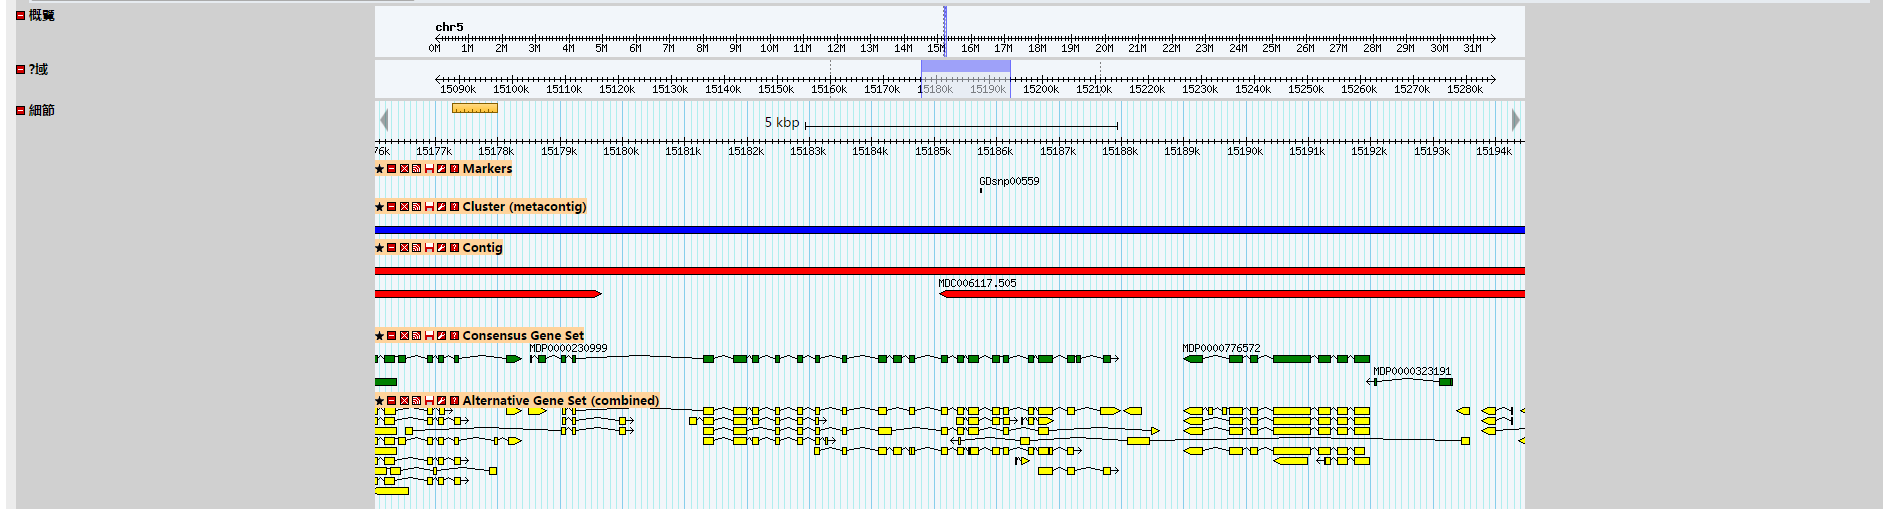
\includegraphics[width = .9\textwidth]{2-1.png}
			\caption{GBrowse页面内容展示图}
		\end{figure}	
		\subsection{系统架构}
			计算机用户必须要树立正确的病毒防范观念,应该对目前互联网上的病毒传播手段有一定的了解,对病毒防范知识要有一定的掌握。互联网中有很多充满诱惑的内容,对于这些极有可能存在病毒的内容,用户必须要增强自己的控制能力,在互联网上下载的各种资料数据在打开和使用之前应该用杀毒软件进行扫描,同时养成良好的计算机操作习惯,这样一来病毒自然就会远离我们。另外,我们还可以通过截断病毒的传播途径来防范病毒。计算机病毒具有极强的传播性,在计算机网络中,如果没有采取有效的防范措施来阻挡其传播途径,那么病毒就会在很短的时间内对局域网、服务器、互联网造成危害。如果处于一个局域网中的某一台计算机受到感染,那么应该立刻断网,对其进行隔离,终止对于这台计算机共享文件的使用,这样一来就能够很好的切断病毒的传播途径,防止病毒危害其他计算机。
		\begin{figure}[!ht]
			\centering
			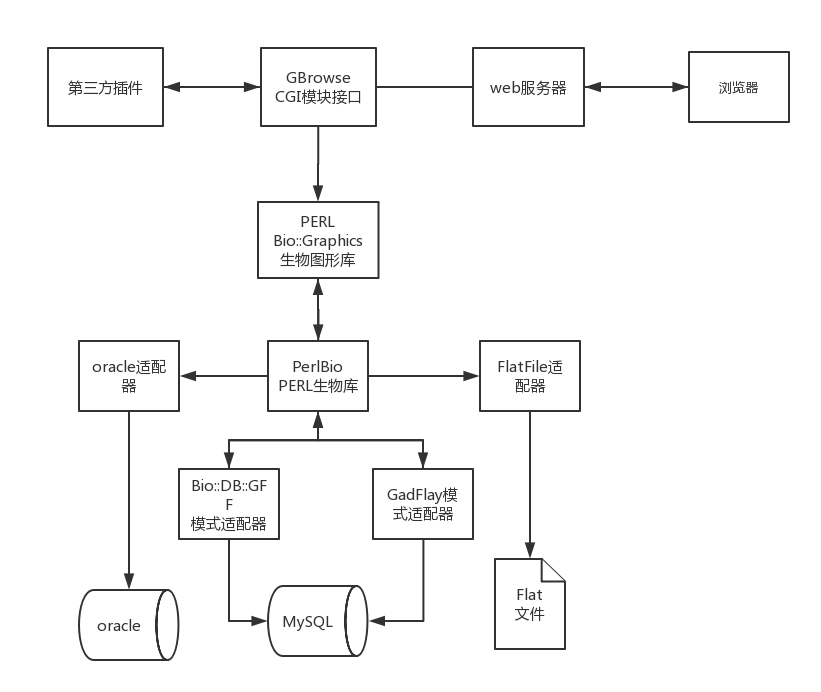
\includegraphics[width = .6\textwidth]{2-2.png}
			\caption{GBrowse系统结构}
		\end{figure}
		\subsection{运行机理}
			计算机用户必须要树立正确的病毒防范观念,应该对目前互联网上的病毒传播手段有一定的了解,对病毒防范知识要有一定的掌握。互联网中有很多充满诱惑的内容,对于这些极有可能存在病毒的内容,用户必须要增强自己的控制能力,在互联网上下载的各种资料数据在打开和使用之前应该用杀毒软件进行扫描,同时养成良好的计算机操作习惯,这样一来病毒自然就会远离我们。另外,我们还可以通过截断病毒的传播途径来防范病毒。计算机病毒具有极强的传播性,在计算机网络中,如果没有采取有效的防范措施来阻挡其传播途径,那么病毒就会在很短的时间内对局域网、服务器、互联网造成危害。如果处于一个局域网中的某一台计算机受到感染,那么应该立刻断网,对其进行隔离,终止对于这台计算机共享文件的使用,这样一来就能够很好的切断病毒的传播途径,防止病毒危害其他计算机。
			\begin{figure}[!ht]
				\centering
				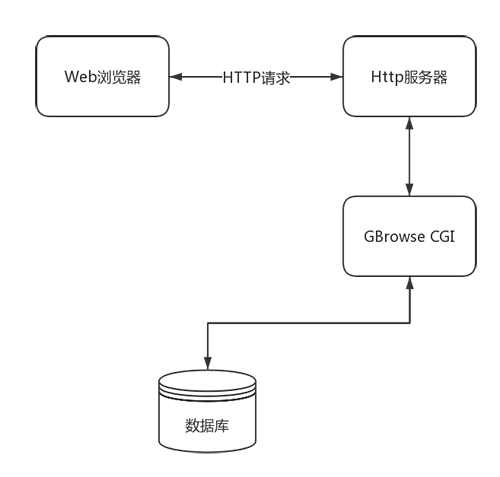
\includegraphics[width = .5\textwidth]{2-3.png}
				\caption{GBrowse模块请求处理}
			\end{figure}
		\subsection{优缺点}
			计算机用户必须要树立正确的病毒防范观念,应该对目前互联网上的病毒传播手段有一定的了解,对病毒防范知识要有一定的掌握。互联网中有很多充满诱惑的内容,对于这些极有可能存在病毒的内容,用户必须要增强自己的控制能力,在互联网上下载的各种资料数据在打开和使用之前应该用杀毒软件进行扫描,同时养成良好的计算机操作习惯,这样一来病毒自然就会远离我们。另外,我们还可以通过截断病毒的传播途径来防范病毒。计算机病毒具有极强的传播性,在计算机网络中,如果没有采取有效的防范措施来阻挡其传播途径,那么病毒就会在很短的时间内对局域网、服务器、互联网造成危害。如果处于一个局域网中的某一台计算机受到感染,那么应该立刻断网,对其进行隔离,终止对于这台计算机共享文件的使用,这样一来就能够很好的切断病毒的传播途径,防止病毒危害其他计算机。
		%JBrowse
	\section{JBrowse}
		\subsection{概述}
			台应用开发框架下逐步推出Windows等操作系统下的应用软件,方便用户可视化数据。
		\subsection{可视化方式}
			JBrowse用 track 的方式进行可视化,提供平滑的动态移动和缩放功能,也有导航和通道的选择。JBrowse可以展示多种 track 视图,除基本视图外,还可以显示非翻译区、外显子、内含子结构等。
		
		\subsection{可视化内容}
			JBrowse可以展示基因组整体视图,也可以细化展示基因跨度、tRNA、转座子、寡核苷酸、蛋白质结合位点、增强子、基因调控区域、非编码RNA、点突变、序列变异信息等其它基因信息。用户可以自己上传需要可视化的内容的相关基因数据,支持GFF、GFF3、WIG、BED、FASTA、Wiggle、BigWig、BAM 等多种格式的数据文件。如图2-5所示
		\begin{figure}[!ht]
			\centering
			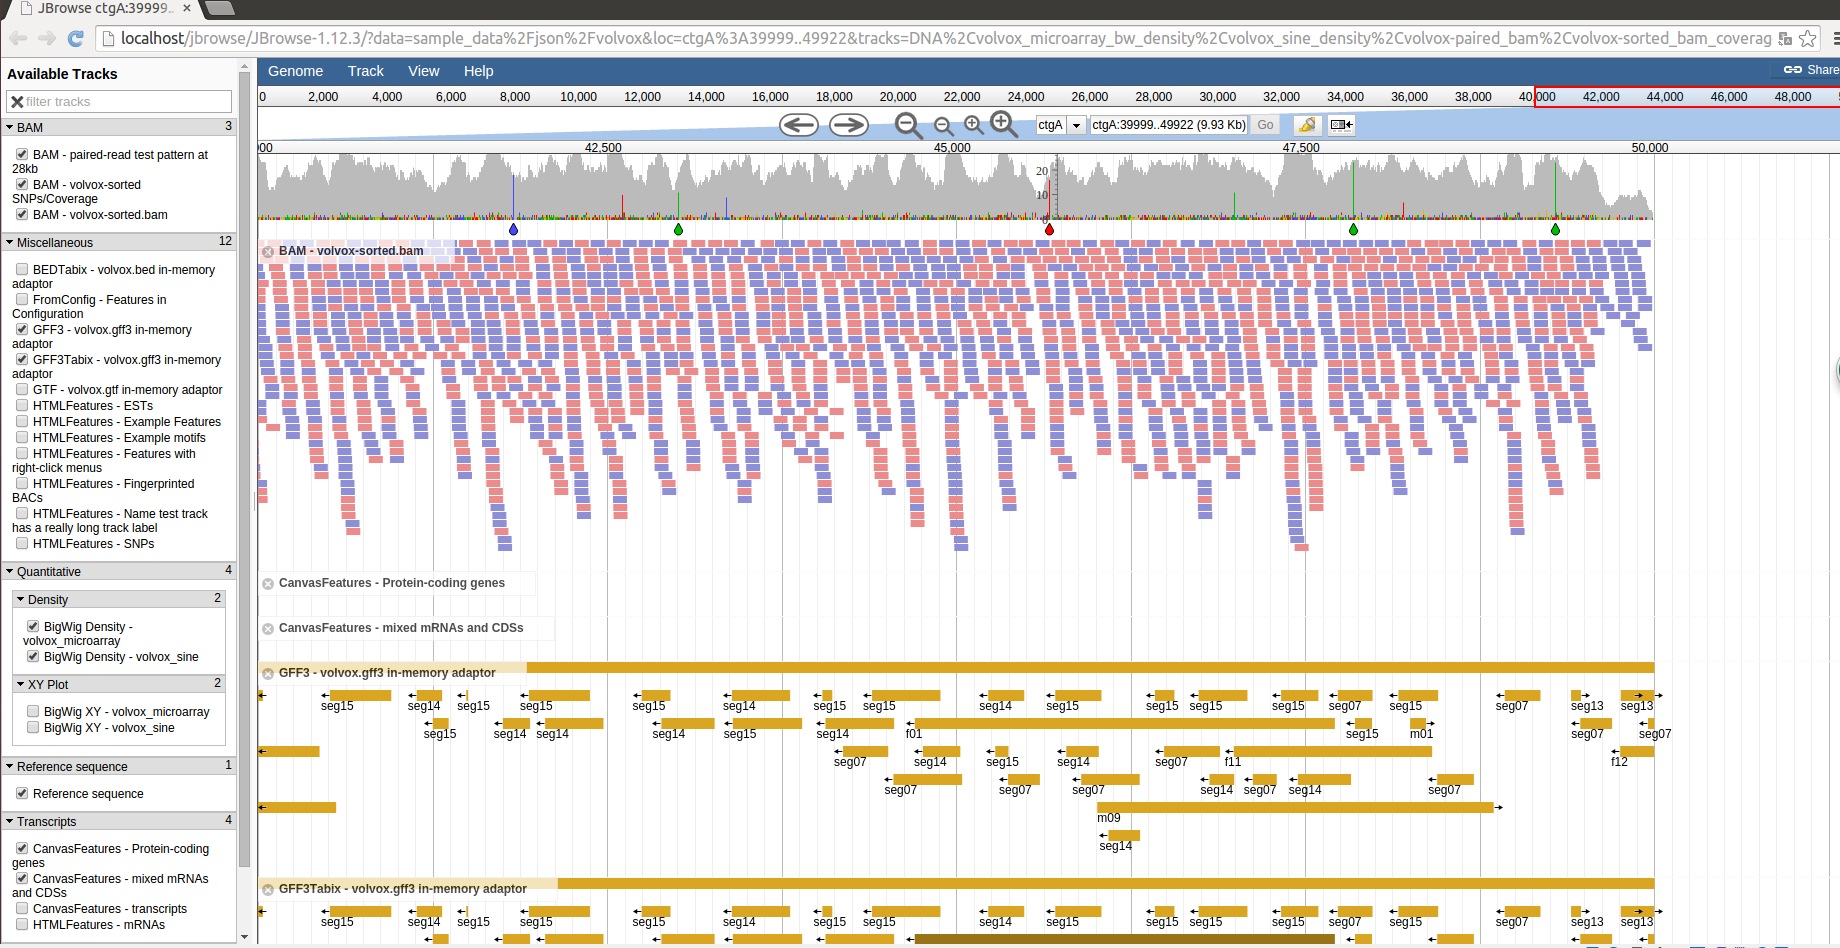
\includegraphics[width = .6\textwidth]{2-4.png}
			\caption{JBrowse可视化内容}
		\end{figure}
		\subsection{系统架构}
			对于计算机病毒的防范,单单依靠技术手段是不能彻底解决问题的,因此必须要把技术和管理结合在一起,这是现阶段病毒防范的主流方法。因为计算机病毒的防范措施,从目前的实际情况来看依旧是非常被动的,人工智能的结合病毒防范技术依旧仅仅停留在实验室阶段,并没有推广和普及。而就网络管理来说,我们可以主动的出击,按照计算机病毒的感染机制,对计算机进行正确的操作和使用,制定完善的网络访问规范,对于服务器进行定期的杀毒和维护,最大限度的预防病毒的侵害。通过对计算机使用的规范化,可以在很大程度上避免用户对不良网站、信息的点击,可以有效的避免一些利用诱惑性图片来吸引用户点击的非法网站,从而预防病毒对计算机的入侵。
		\begin{figure}[!ht]
			\centering
			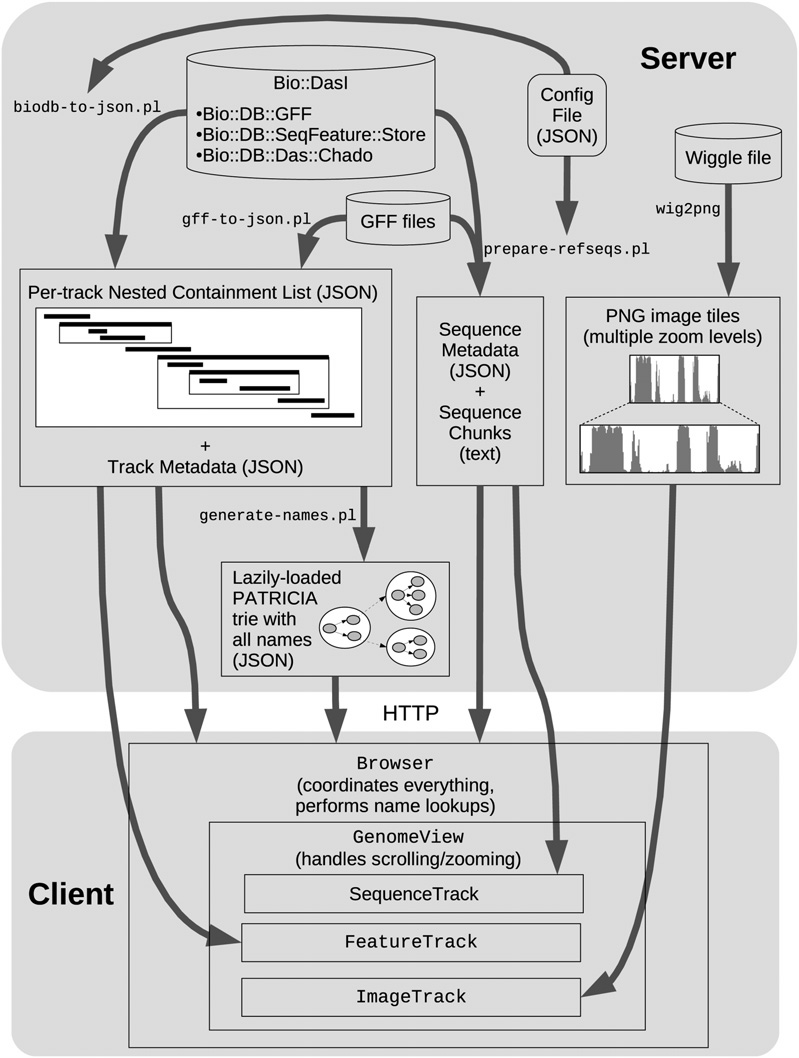
\includegraphics[width = .4\textwidth]{2-5.png}
			\caption{JBrowse系统架构}
		\end{figure}
		\subsection{运行机理}
		第一,导致计算机运行缓慢。当病毒程序执行的过程中,不但会占据计算机内存,还会干扰系统的正常运行,导致系统运行缓慢。虽然说这样的危害从表面上来看并不会给系统带来较大的损失,但是在用户使用计算机的过程中,会不断的消耗计算机系统的资源,最终甚至可能导致系统的停止运行。

		第二,病毒会大量占用系统内存以及计算机磁盘空间。当计算机感染某些病毒之后,硬盘会自动开始持续性的读取,虽然用户并未执行操作,但是硬盘却处于高速运转状态,计算机内存也被大量的占用。此外,某些文件型病毒甚至可能在短时间内感染大量的系统文件,从而让用户硬盘中产生大量的垃圾文件,极大的占据了硬盘空间。

		第三,对计算机数据进行破坏。病毒极有可能篡改计算机系统设置或者对计算机系统进行加密的方法,从而引起计算机系统的混乱,更严重的时候会破坏计算机的硬盘引导区,造成计算机无法正常启动等。第四,病毒所带来的垃圾信息会对用户计算机网络造成一定的危害,甚至可能导致网络瘫痪现象。例如当计算机感染蠕虫病毒之后,在用户不知情的情况下,病毒会让计算机向外发送大量垃圾邮件或数据,从而让网络严重堵塞或瘫痪。最近几年以来,很多不法分子通过即时通讯软件向用户发送大量带有病毒的垃圾信息和邮件,成为了病毒传播的一种新的途径。

		第五,窃取用户的各种隐私。当前,很多计算机用户对于木马病毒已经是深恶痛绝。有关调查显示,当前木马病毒占据了计算机病毒的60\%左右,其中大部分木马病毒的传播目的都是为了窃取用户的个人信息从而帮助病毒制造者获取非法利益。用户信息一旦泄露,将会给用户带来不可估量的损失。
		\begin{figure}[!ht]
			\centering
			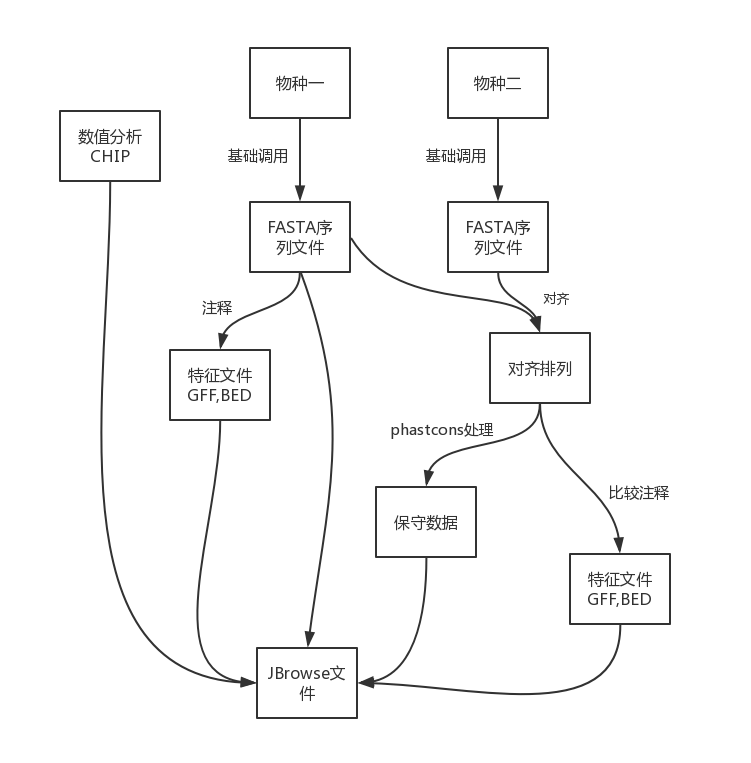
\includegraphics[width = .4\textwidth]{2-6.png}
			\caption{JBrowse工作流图}
		\end{figure}
		\subsection{优缺点}
		优点:流浏览器对 HTML5 中新标签的支持不完善,造成用户体验不佳等问题。
	\section{UCSC Genome Browser}		
			\subsection{概述}	
			 按照病毒的存在媒体进行分类,一般可以分为引导型、文件型和混合型三种类型。引导型病毒一般来说主要藏匿于磁盘引导区,当电脑启动之后,隐藏在磁盘的病毒便会开始传播;文件型的病毒常常会对计算机中的可执行文件进行感染,例如com、exe、doc文件;而混合型病毒属于上述两种病毒的混合型,其算法复杂,传播的途径和危害更大。
			\subsection{可视化方式}		
			 按照病毒的存在媒体进行分类,一般可以分为引导型、文件型和混合型三种类型。引导型病毒一般来说主要藏匿于磁盘引导区,当电脑启动之后,隐藏在磁盘的病毒便会开始传播;文件型的病毒常常会对计算机中的可执行文件进行感染,例如com、exe、doc文件;而混合型病毒属于上述两种病毒的混合型,其算法复杂,传播的途径和危害更大。
			\begin{figure}[!ht]
				\centering
				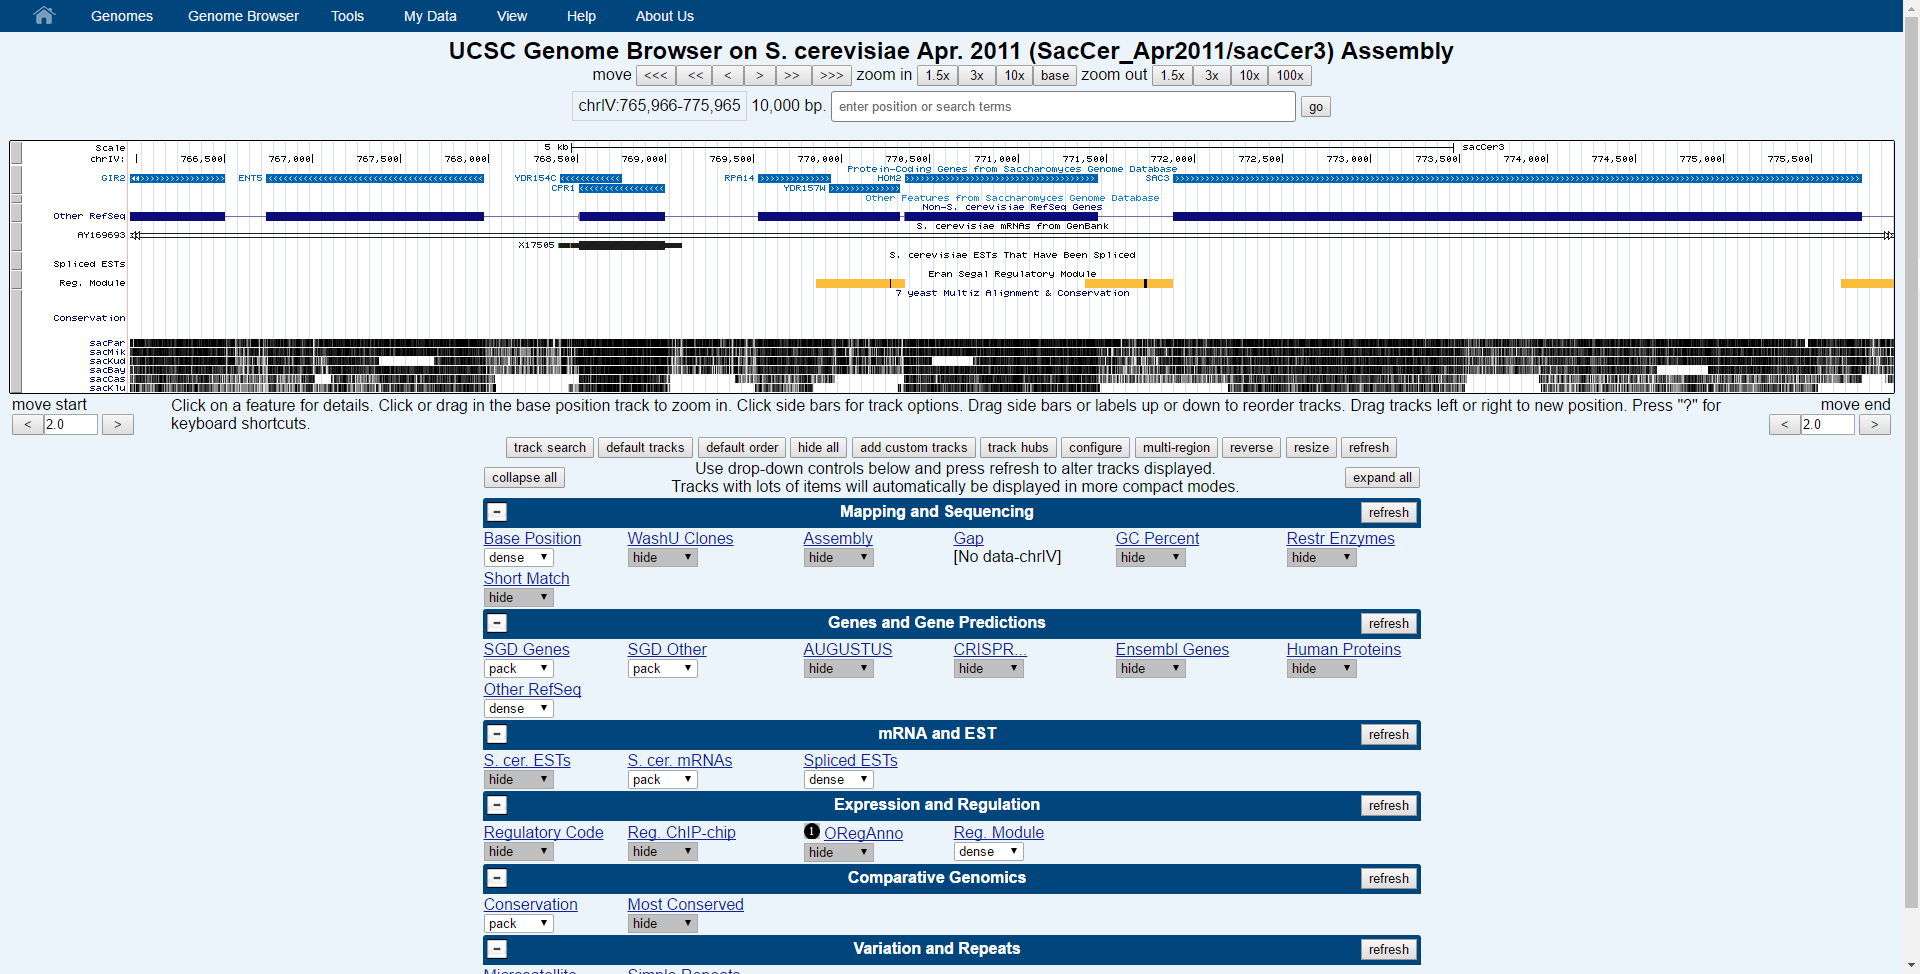
\includegraphics[width = .4\textwidth]{2-7.png}
				\caption{UCSC Genome Browser系统界面}
			\end{figure}
			\subsection{可视化内容}		
			 按照病毒的存在媒体进行分类,一般可以分为引导型、文件型和混合型三种类型。引导型病毒一般来说主要藏匿于磁盘引导区,当电脑启动之后,隐藏在磁盘的病毒便会开始传播;文件型的病毒常常会对计算机中的可执行文件进行感染,例如com、exe、doc文件;而混合型病毒属于上述两种病毒的混合型,其算法复杂,传播的途径和危害更大。
			\subsection{系统架构}		
			工作站是直接面向互联网的,大多数的病毒都是首先通过工作站传播到整个网络中去的。现阶段工作站对病毒的防范措施主要有三种:第一是软件防范,这种防范方法相对简单,它通过在工作站上安装最新的杀毒软件就能够起到预防病毒入侵的目的。需要注意的是,使用这种方法必须要及时的对杀毒软件的病毒库进行升级,这样才能够预防更多的已知病毒;第二是在工作站上插入病毒卡,选择这种病毒防范措施的有点是可以实现对病毒入侵的实时监测,进一步的增强工作站病毒防范能力。但是这种方式的缺点也比较突出,它会占据一部分系统资源,从而导致系统运行速度变慢,而且病毒卡的升级更新相对来说也比较困难;第三是在网络接口上装病毒防御芯片,它可以把工作站与服务器的存储控制和病毒防御结合在一起,进一步增强计算机病毒的实时防御。另外这种防范措施也在一定程度上增强了服务器的安全性,但是这种方法也存在一个升级更新不便的问题。因此当前选择最多的防范措施依旧是安装杀毒软件。
			\subsection{优缺点}
			计算机病毒属于人为编写的,直接感染计算机系统同时对系统资产造成危害的一种程序,从本质上来说计算机病毒属于一个拥有自我复制能力的程序,它会对计算机软硬件造成较大的危害。病毒的种类非常多,而不同类型的病毒其危害程度和感染方式也不尽相同。一般来说我们主要将计算机病毒分为以下几种类型:
	\chapter{基因组浏览器环境搭建与配置}
	\chaptermark{基因组浏览器环境搭建与配置}
	\section{GBrowse搭建与配置}
	虽然计算机病毒危害大,传播快,但是只要普通用户能够树立正确的防范意识,积极做好各种计算机病毒防范措施,还是可以在很大程度上避免病毒对计算机造成的危害,确保互联网的安全。虽然说新病毒层出不穷,病毒也越来越隐蔽,现有的计算机操作系统本身也还存在着一定的缺陷和漏洞,很多新型的病毒能够利用这些漏洞在互联网中传播。但是只要每一个用户都能够提高反病毒的警惕性,通过科学有效的病毒防御方法,新出现的各种病毒就不会对用户造成大的威胁。当我们的计算机发现病毒之后,我们所安装的反病毒防御系统能够第一时间展开防御。我们有理由相信,随着病毒防御技术的不断提升以及用户病毒防范意识的提升,计算机病毒的生存空间必然会越来越小。
	\subsection{服务端平台选取及环境需求}
	虽然计算机病毒危害大,传播快,但是只要普通用户能够树立正确的防范意识,积极做好各种计算机病毒防范措施,还是可以在很大程度上避免病毒对计算机造成的危害,确保互联网的安全。虽然说新病毒层出不穷,病毒也越来越隐蔽,现有的计算机操作系统本身也还存在着一定的缺陷和漏洞,很多新型的病毒能够利用这些漏洞在互联网中传播。但是只要每一个用户都能够提高反病毒的警惕性,通过科学有效的病毒防御方法,新出现的各种病毒就不会对用户造成大的威胁。当我们的计算机发现病毒之后,我们所安装的反病毒防御系统能够第一时间展开防御。我们有理由相信,随着病毒防御技术的不断提升以及用户病毒防范意识的提升,计算机病毒的生存空间必然会越来越小。
	\subsection{源码编译安装Apache与MySQL}
		\subsubsection{(1)数学公式}
		
		\subsubsection{(2)源码编译的步骤}
		
		\begin{lstlisting}[language=bash]
		groupadd apache
		useradd -g apache apache -s /bin/false
		groupadd mysql
		useradd -g mysql mysql -s /bin/false
		\end{lstlisting}
		\begin{table}[!htbp]
			\centering
			\begin{tabular}{ll}	
				\toprule
				选项名称& 含义\\
				\midrule
				--build&定义正在构建工具的系统的系统类型。它默认为脚本的结果 config.guess。\\
				--host&定义服务器运行的系统的系统类型。 HOST默认为BUILD。\\
				--target&为系统类型TARGET构建编译器 。它默认为HOST。\\
				--prefix& 指定Apache的安装目录前缀\\
				--enable-module&相应的模块将构建为DSO模块\\
				--enable-deflate&开启网页压缩\\
				--enable-rewrite&开启http重写\\
				--enable-file-cache&开启文件缓存\\
				--enable-cache&开启缓存\\
				\bottomrule
			\end{tabular}
		\caption{Apache选项参数}
		\end{table}
	
	\chapter{数学公式测试}
\chaptermark{数学公式测试}
	\section{数学公式测试}
		\subsection{数学公式测试}
		\begin{equation}
		\forall x \in \mathbf{R}:
		\qquad x^{2} \geq 0
		\end{equation}
		\begin{equation}
		\forall x \in \mathbf{R}:
		\qquad x^{2} \geq 0
		\end{equation}
		\begin{equation}
		\forall x \in \mathbf{R}:
		\qquad x^{2} \geq 0
		\end{equation}
		\subsection{数学公式测试}
	
	
	



			
	%\include{pagers/chapter5}
	%\include{pagers/chapter6}
	\newpage
	%参考文献
	\addcontentsline{toc}{chapter}{参考文献}
\chaptermark{参考文献}
\nocite{*}
\printbibliography[title=参考文献]
	%致谢
	\chapter*{致谢}
\addcontentsline{toc}{chapter}{致谢}

时间如白驹过隙,四年的大学生活转眼就结束了。

在这短短的四年里,经历了许许
多多的事情,有快乐有悲伤,也曾遇到挫折也曾彷徨,好在身旁有许许多多帮助我的人,
首先感谢我的导师于建涛老师, 于老师工作十分负责,非常关注我的毕业设计进度
并且在遇到困难的时候给予我思路和方向, 于老师严谨细致的工作作风一直伴随着我整
个毕业设计的过程,时刻激励着我对整个毕业设计的改进和优化。在此, 我非常感谢于
老师对我的毕业设计和论文的帮助和支持。

感谢我的舍友们,在这四年里是你们一直陪伴在我的身边,在我遇到困难的时候伸
出援手帮助我度过难关。

感谢我的爸爸妈妈, 无论什么时候都爸爸妈妈在背后默默支持我、鼓励我,让我顺
利的完成了学业,并将继续支持我出国深造,是你们的支持给予了我前进的动力, 让我
有力量继续走下去。

现在论文即将完成,心情很是激动,回想起从一开始的选题到现在论文的完成,我
经历了许许多多,在这期间也有许许多多的人给予我无私的帮助,在此请接受我最诚挚
的感谢。

\fancypagestyle{plain}{
	\fancyhf{}
	\fancyhead[CE]{致谢}
	\fancyhead[CO]{致谢}
	\fancyfoot[C]{-\thepage-}
}
\end{document}